\chapter{Modelle}
\section{Szenarios}
\subsection{Überwachung und Messung an einem Versuchsaufbau}
\subsection{Steuerung und Messung an einem Versuchsaufbau}
\section{Use case model}
Dieses Use case Diagramm zeigt die dem Nutzer zu Verfügung stehen Optionen.
\begin{figure}[H]
 \centering
 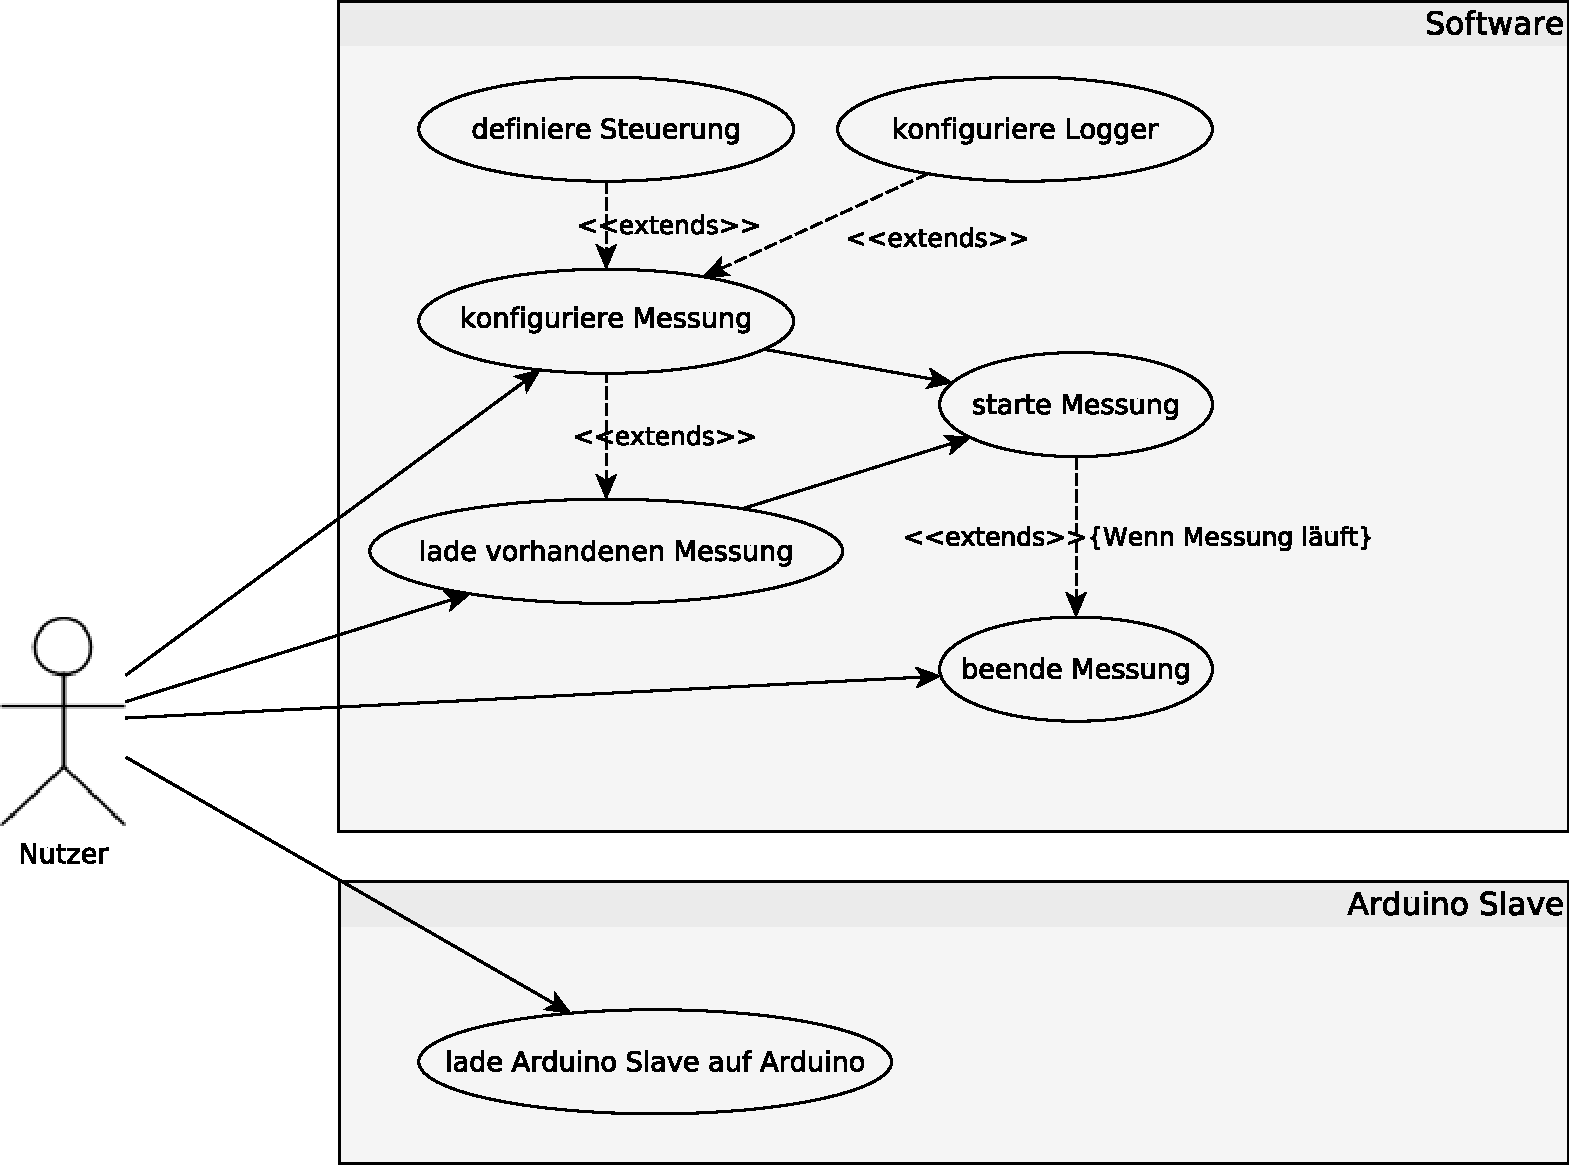
\includegraphics[width=\textwidth, keepaspectratio=true]{../Diagramme/BachelorUseCase1.pdf}
\end{figure}

%\section{Analysis object model}
%\section{Dynamic model}
\section{Flowchart}
Dieses Flowchart zeigt die notwendigsten Schritte, die von der Software und dem Nutzer unternommen werden müssen um eine erfolgreiche Messung durch führen zu können. 
\begin{figure}[H]
 \centering
 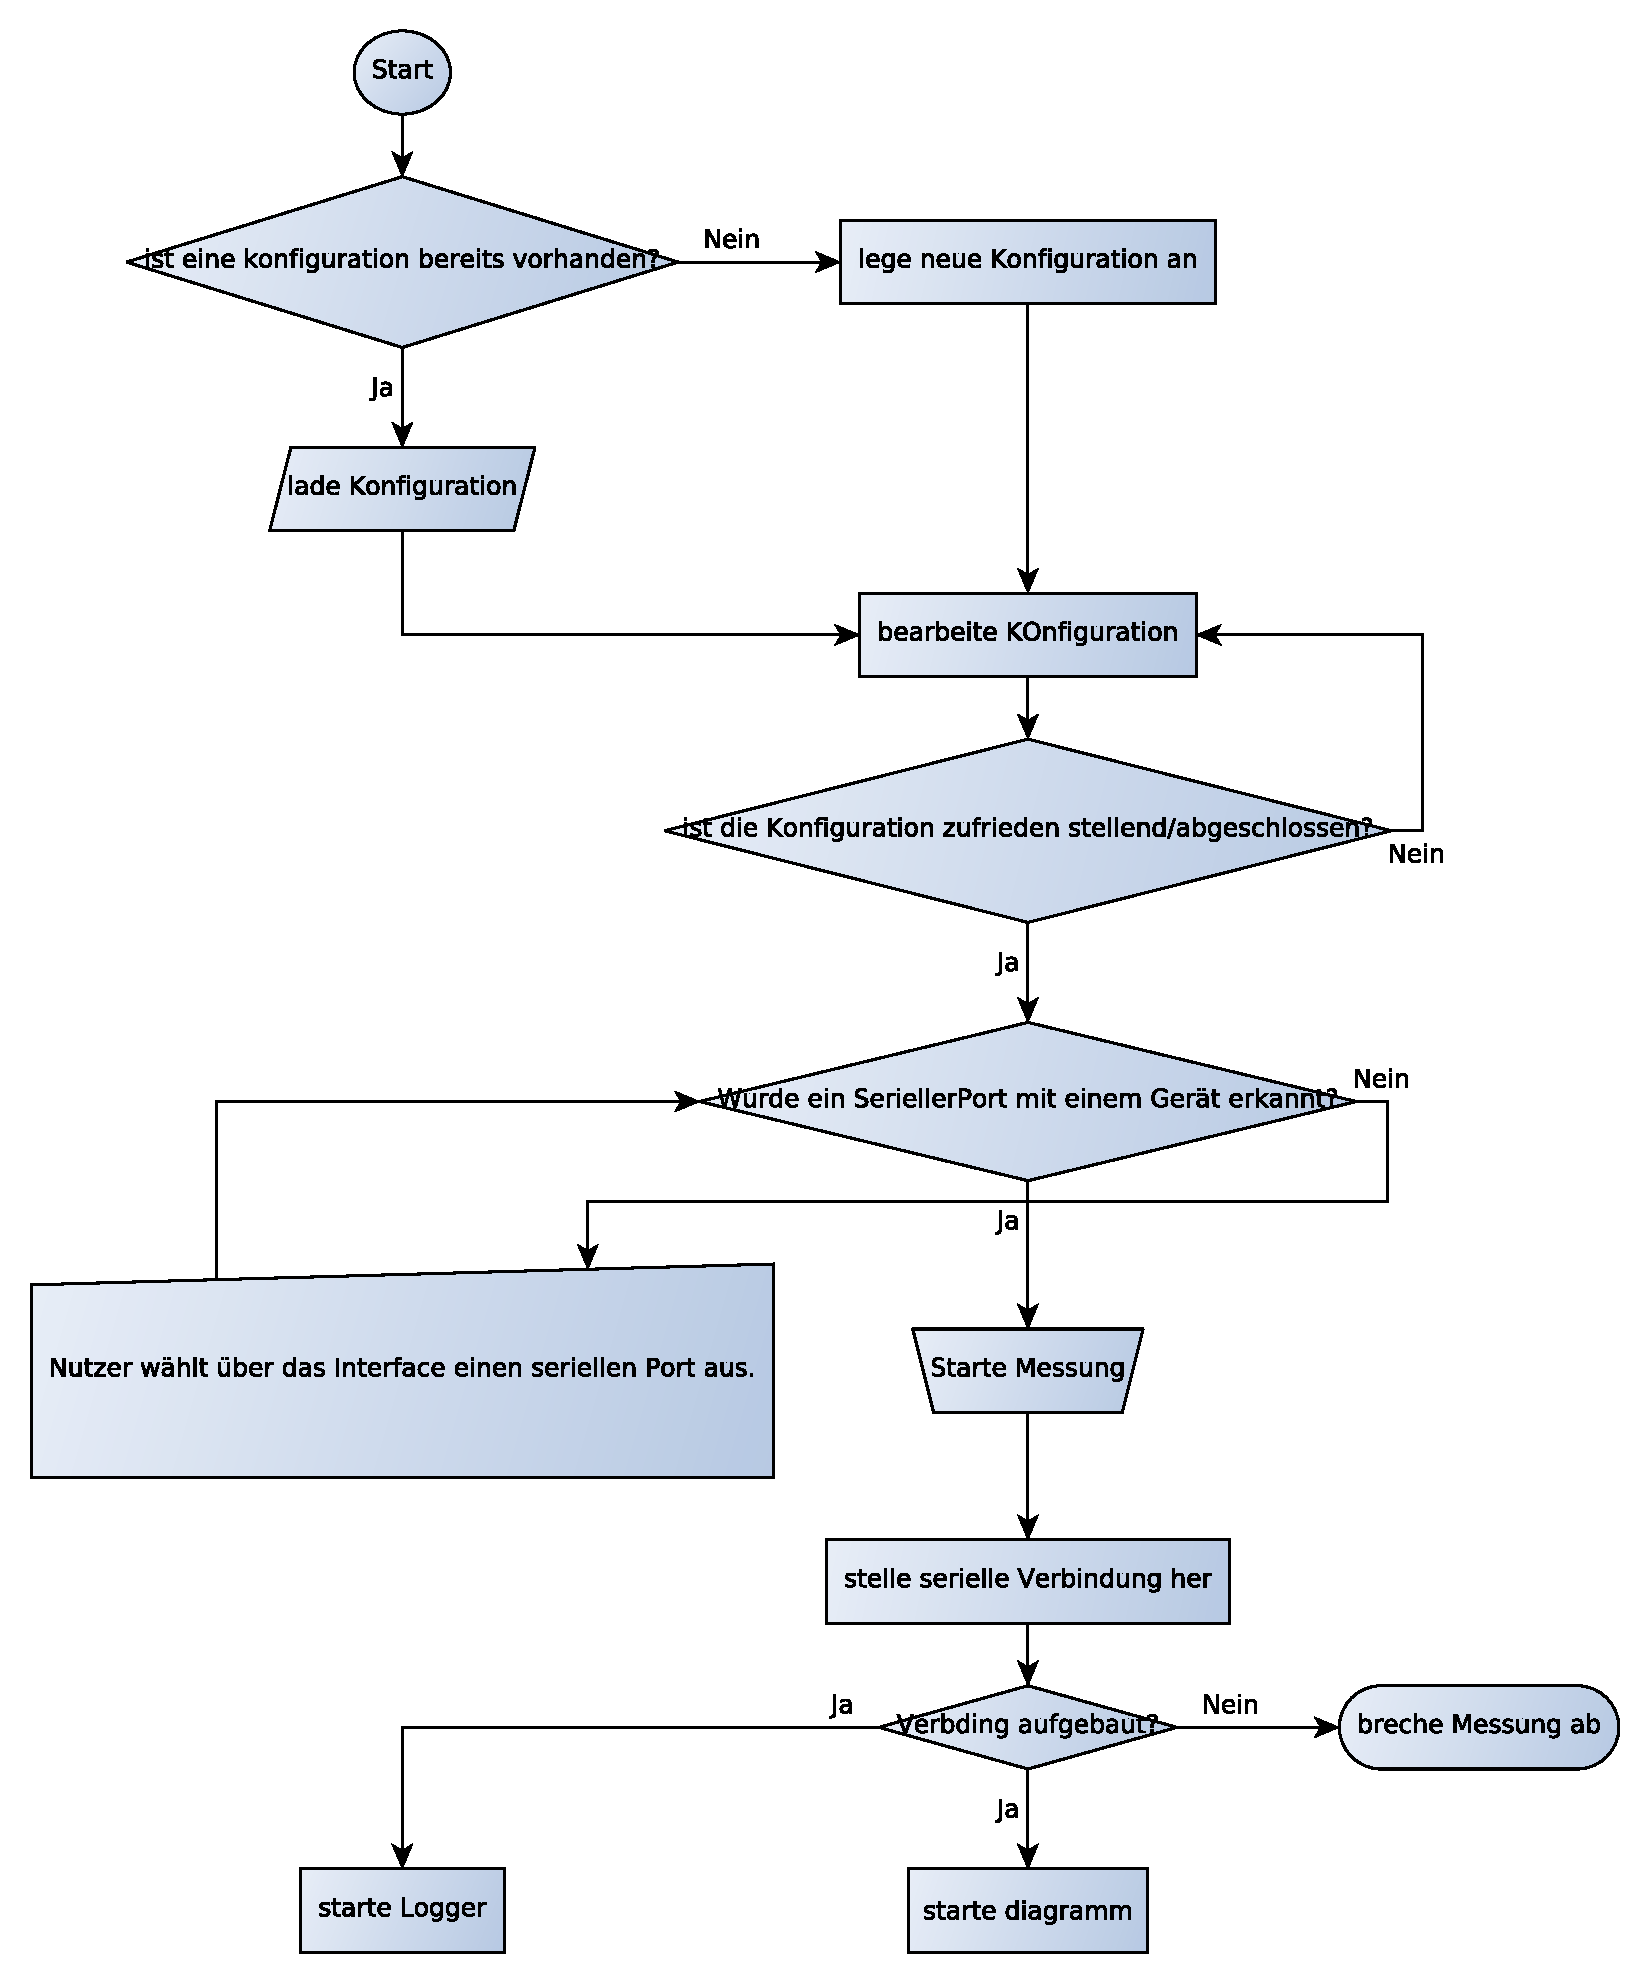
\includegraphics[width=\textwidth, keepaspectratio=true]{../Diagramme/SoftwareFlowChart.pdf}
\end{figure}
\section{Aufbau}
%grobes UML
\section{User Interface - Navigation und Mockups}